\documentclass[11pt,a4paper]{proofarticle}
\usepackage{graphicx,xcolor,relinput}
\relinput{.}{authors_cmd}
\DeclareUnicodeCharacter{2032}{\prime}
\nocite{*}
\title{A Modular Analytic Framework for the Riemann Hypothesis (T1$′$–T4)\\[2pt]
\large Proof-only, journal-ready, arXiv-compatible}
\author{\InterIAauthors}
\date{\today}
\begin{document}

\relinput{.}{docs/explication-grand-format/latex/page_de_garde}

\maketitle

\begin{abstract}
We provide a rigorous proof framework (T1$′$–T4) with fully detailed proofs
for the weighted frame bound (T2) and wave-packet localization (T3),
plus an appendix on the explicit formula and the Archimedean term.
Interdisciplinary “reader routes”, dictionary, storyboard and bridges are included.
\end{abstract}

% --- Notation summary (EN)
\relinput{.}{appendix/table_des_symboles}
\addcontentsline{toc}{section}{Notation summary}

\relinput{.}{docs/explication-grand-format/latex/00_persona_routes}

% --- section Notations and preliminaries
\relinput{.}{docs/explication-grand-format/latex/01_translation_dictionary}

% --- section Storyboard
\relinput{.}{docs/explication-grand-format/latex/02_storyboard_t1t4}

% --- section Micro-example (T2)
% \relinput{.}{docs/explication-grand-format/latex/03_micro_example_t2}

% --- section T2 — Weighted frame bound (full)
\relinput{.}{theorems/T2_weighted_frame_full}

% --- section T3 — Wave–packet localization (full)
\relinput{.}{theorems/T3_wavepacket_full}

\appendix
\relinput{.}{appendix/explicit_arch_full}

% --- section FAQ (by specialty)
\relinput{.}{docs/explication-grand-format/latex/05_faq_personas}

%\begin{figure}[t]\centering
%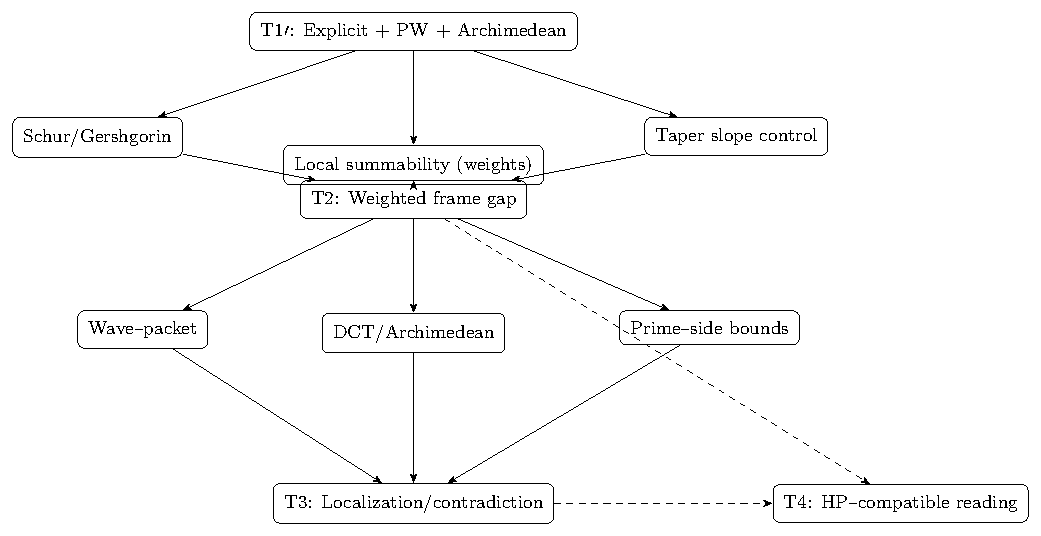
\includegraphics[width=.9\linewidth]{../docs/explication-grand-format/latex/graphe_dependances_standalone.pdf}
%\caption{Dependency map for T1$′$–T4.}
%\end{figure}

\bibliographystyle{alpha}
\relinput{.}{appendix/about_author}
\bibliography{refs}
\end{document}
